\documentclass[11pt]{article}
\usepackage[notes]{la}
\lamodule{1}{3}{Vector Equations}
\laxdoc{1.1}   % cross-references to Section 1.1 as \ref{1.1-<label>}
\laxdoc{1.2}   % cross-references to Section 1.2 as \ref{1.2-<label>}

\begin{document}

\section{Vector Equations}

\begin{guide}
A linear system lists many constraints on many unknown \emph{numbers}. Can all of those constraints be
packed into a \emph{single} equation about a single unknown \emph{list} of numbers? And if they can, what
does it mean, geometrically, to solve that one equation?
\end{guide}

\textbf{By the end of this section you should be able to:}
\begin{itemize}
  \item add vectors and multiply them by scalars, entry by entry and (in $\R^2$) geometrically;
  \item form linear combinations, and say what the \emph{weights} are;
  \item rewrite a linear system as a vector equation and back, and read the augmented matrix directly from the vectors;
  \item decide whether a vector is a linear combination of given vectors, and find the weights when it is;
  \item define $\Span\{\bv{v}_1,\dots,\bv{v}_p\}$, describe it geometrically, and find the equation that
        a vector must satisfy to lie in it;
  \item explain why the weights in a linear combination need not be unique.
\end{itemize}

% ---------------------------------------------------------------------
\subsection*{Vectors in $\R^n$}

Until Chapter~4, the word \emph{vector} will mean an \emph{ordered list of numbers}, written as a column. A matrix
with one column is called a \emph{column vector}, or simply a \emph{vector}. For example,
\[
\bv{u}=\begin{bmatrix}3\\-1\end{bmatrix},\qquad
\bv{v}=\begin{bmatrix}1\\0\\5\end{bmatrix},\qquad
\bv{w}=\begin{bmatrix}w_1\\w_2\end{bmatrix}\ \ (w_1,w_2 \text{ any real numbers}).
\]

\begin{defn}{Vectors in $\R^n$ and their algebra}{vectors}
For a positive integer $n$, $\R^n$ (read ``r-n'') is the set of all vectors with $n$ real entries,
\[
\bv{u}=\begin{bmatrix}u_1\\ \vdots\\ u_n\end{bmatrix}.
\]
Two vectors in $\R^n$ are \emph{equal} if and only if their corresponding entries are equal. The \emph{sum} of
$\bv{u}$ and $\bv{v}$ and the \emph{scalar multiple} of $\bv{u}$ by a real number (a \emph{scalar}) $c$ are defined
\emph{entry by entry}:
\[
\bv{u}+\bv{v}=\begin{bmatrix}u_1+v_1\\ \vdots\\ u_n+v_n\end{bmatrix},\qquad
c\,\bv{u}=\begin{bmatrix}cu_1\\ \vdots\\ cu_n\end{bmatrix}.
\]
The \emph{zero vector} $\bv{0}$ has all entries $0$. We write $-\bv{u}$ for $(-1)\bv{u}$ and
$\bv{u}-\bv{v}$ for $\bv{u}+(-1)\bv{v}$.
\end{defn}

To save space we sometimes write a column vector as $(3,-1)$. The parentheses and the comma distinguish it from the
$1\times2$ row matrix $\begin{bmatrix}3&-1\end{bmatrix}$; a column and a row with the same entries are
\emph{different} objects, because they have different shapes. Two vectors with different numbers of entries are never
equal and can never be added.

\begin{kc}{Compute}{compute}
Let $\bv{u}=(2,-1)$ and $\bv{v}=(-1,3)$. Compute $3\bv{u}+2\bv{v}$ and $\bv{u}-\bv{v}$.
\end{kc}

\begin{kc}{One vector equation, two numbers}{vecequal}
Find the numbers $x$ and $y$ for which
\[
x\begin{bmatrix}1\\1\end{bmatrix}+y\begin{bmatrix}1\\-1\end{bmatrix}=\begin{bmatrix}5\\1\end{bmatrix}.
\]
(Hint: what does ``equal'' mean for vectors?)
\end{kc}

The operations obey the familiar rules of arithmetic.

\begin{thm}{Algebraic properties of $\R^n$}{props}
For all $\bv{u},\bv{v},\bv{w}$ in $\R^n$ and all scalars $c,d$:
\begin{enumerate}[label=(\roman*),itemsep=1pt]
  \item $\bv{u}+\bv{v}=\bv{v}+\bv{u}$
  \item $(\bv{u}+\bv{v})+\bv{w}=\bv{u}+(\bv{v}+\bv{w})$
  \item $\bv{u}+\bv{0}=\bv{u}$
  \item $\bv{u}+(-\bv{u})=\bv{0}$
  \item $c(\bv{u}+\bv{v})=c\bv{u}+c\bv{v}$
  \item $(c+d)\bv{u}=c\bv{u}+d\bv{u}$
  \item $c(d\bv{u})=(cd)\bv{u}$
  \item $1\bv{u}=\bv{u}$
\end{enumerate}
\end{thm}

\begin{proof}
Each property is a statement about \emph{vectors}, and vectors are equal when their entries are equal, so each
reduces to the corresponding property of real numbers, one entry at a time. For (i): the $i$th entry of
$\bv{u}+\bv{v}$ is $u_i+v_i$, which equals $v_i+u_i$, the $i$th entry of $\bv{v}+\bv{u}$. For (v): the $i$th entry of
$c(\bv{u}+\bv{v})$ is $c(u_i+v_i)=cu_i+cv_i$, the $i$th entry of $c\bv{u}+c\bv{v}$. The remaining six properties are
checked in exactly the same way (you will do two of them in the homework).
\end{proof}

\begin{think}{What would another world of ``vectors'' need?}{axioms}
Imagine a different collection of objects (polynomials of degree at most $2$, say, or $2\times2$ matrices) with some
rule for adding two of them and multiplying one by a scalar. The eight properties above are what made $\R^n$ pleasant
to calculate in. Which of the eight would you check to decide whether the new collection behaves like $\R^n$?
Can you find a collection of vectors in $\R^2$ for which a few of the eight \emph{fail}? (Try ``all vectors in $\R^2$
with positive entries''.)
\end{think}

% ---------------------------------------------------------------------
\subsection*{Geometry of $\R^2$}

A vector $(a,b)$ in $\R^2$ is identified with the point $(a,b)$ in the plane, and we often draw an arrow from the origin to
that point. Vector addition then has a picture.

\begin{center}
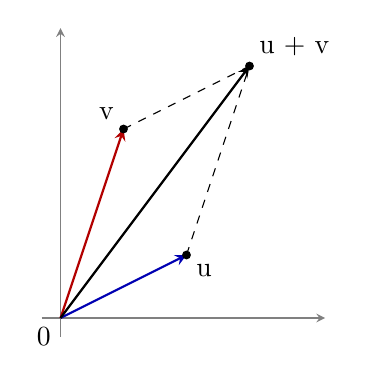
\begin{tikzpicture}[scale=0.8,>=stealth]
  \draw[->,gray] (-0.3,0)--(4.2,0); \draw[->,gray] (0,-0.3)--(0,4.6);
  \draw[->,thick,blue!70!black] (0,0)--(2,1);
  \draw[->,thick,red!70!black] (0,0)--(1,3);
  \draw[->,thick] (0,0)--(3,4);
  \draw[dashed] (2,1)--(3,4); \draw[dashed] (1,3)--(3,4);
  \fill (2,1) circle (2pt); \fill (1,3) circle (2pt); \fill (3,4) circle (2pt);
  \node[below right] at (2,1) {u};
  \node[above left] at (1,3) {v};
  \node[above right] at (3,4) {u + v};
  \node[below left] at (0,0) {0};
\end{tikzpicture}
\end{center}

For $\bv{u}=(2,1)$ and $\bv{v}=(1,3)$ we get $\bv{u}+\bv{v}=(3,4)$: the fourth vertex of the parallelogram whose other
vertices are $\bv{0},\bv{u},\bv{v}$. This is the \emph{parallelogram rule}. (It holds because the side from $\bv{v}$ to
$\bv{u}+\bv{v}$ is a copy of the side from $\bv{0}$ to $\bv{u}$ moved by $\bv{v}$, and the same with the roles reversed.)
Multiplying by a scalar $c$ stretches the arrow by the factor $|c|$ and reverses it when $c<0$. In particular, the set of
\emph{all} scalar multiples of a nonzero vector $\bv{u}$ is the line through the origin and $\bv{u}$.

\begin{think}{Arrow or list?}{arrow}
In $\R^5$ you cannot draw an arrow. So in what sense is the picture ``true'' in $\R^2$ and still useful in $\R^5$?
Also: the arrow from $\bv{0}$ to $\bv{u}$ and the arrow from $\bv{v}$ to $\bv{u}+\bv{v}$ have the same length and direction.
Does the vector $\bv{u}$ ``live'' at a particular place? Finally, draw $\bv{u}$, $\bv{v}$ and $\bv{u}-\bv{v}$ for the vectors above and
explain where the arrow for $\bv{u}-\bv{v}$ points.
\end{think}

% ---------------------------------------------------------------------
\subsection*{Linear combinations}

\begin{defn}{Linear combination and weights}{lincomb}
Given vectors $\bv{v}_1,\dots,\bv{v}_p$ in $\R^n$ and scalars $c_1,\dots,c_p$, the vector
\[
\bv{y}=c_1\bv{v}_1+c_2\bv{v}_2+\cdots+c_p\bv{v}_p
\]
is called a \emph{linear combination} of $\bv{v}_1,\dots,\bv{v}_p$ with \emph{weights} $c_1,\dots,c_p$.
Any real number, including $0$, may be used as a weight.
\end{defn}

By Theorem~\ref{thm:props}(ii) we may omit parentheses in a linear combination.

\begin{exmp}{Computing linear combinations}{compute}
Let $\bv{v}_1=(1,-2,3)$ and $\bv{v}_2=(4,0,-1)$. Then
\[
2\bv{v}_1-3\bv{v}_2=\begin{bmatrix}2\\-4\\6\end{bmatrix}+\begin{bmatrix}-12\\0\\3\end{bmatrix}
=\begin{bmatrix}-10\\-4\\9\end{bmatrix},\qquad
\bv{v}_1+\bv{v}_2=\begin{bmatrix}5\\-2\\2\end{bmatrix}.
\]
Using weights $0$ and $0$ gives the zero vector, and using weights $1$ and $0$ gives $\bv{v}_1$ itself. So both of the vectors
$\bv{v}_1$ and $\bv{v}_2$, and the zero vector, are linear combinations of $\bv{v}_1,\bv{v}_2$.
\end{exmp}

The interesting question runs the other way. We are \emph{given} a vector $\bv{b}$ and ask: \emph{which weights, if any,
produce it?} The weights are the unknowns, so we must solve an equation. We start from a system of equations and
repackage it.

\begin{exmp}{A system as one vector equation}{translate}
Consider
\[
\begin{aligned}
2x_1+\phantom{3}x_2-x_3&=\phantom{-}3\\
x_1-3x_2+4x_3&=-2.
\end{aligned}
\]
Two vectors are equal exactly when both of their entries are equal, so this pair of equations says the same thing as the
single equation
\[
\begin{bmatrix}2x_1+x_2-x_3\\ x_1-3x_2+4x_3\end{bmatrix}=\begin{bmatrix}3\\-2\end{bmatrix}.
\]
The vector on the left splits into a sum with one term for each unknown, and each term is a scalar times a column of
coefficients:
\[
x_1\begin{bmatrix}2\\1\end{bmatrix}+x_2\begin{bmatrix}1\\-3\end{bmatrix}+x_3\begin{bmatrix}-1\\4\end{bmatrix}
=\begin{bmatrix}3\\-2\end{bmatrix}.
\]
This is a \emph{vector equation}. In this language, a solution is a list of weights. For instance,
$(x_1,x_2,x_3)=(1,1,0)$ works, because
$1\cdot(2,1)+1\cdot(1,-3)+0\cdot(-1,4)=(3,-2)$. The system has three unknowns and only two equations and is consistent,
so by Theorem~\ref{1.2-thm:counting}(c) it has infinitely many solutions: there are many different ways to build
$(3,-2)$ from these three columns.
\end{exmp}

The pattern in Example~\ref{ex:translate} is completely general, and so is the proof.

\begin{thm}{Vector equations and linear systems}{vecsys}
Let $\bv{a}_1,\dots,\bv{a}_n$ and $\bv{b}$ be vectors in $\R^m$. The vector equation
\[
x_1\bv{a}_1+x_2\bv{a}_2+\cdots+x_n\bv{a}_n=\bv{b}
\]
has the same solution set as the linear system whose augmented matrix is
\[
\begin{bmatrix}\bv{a}_1&\bv{a}_2&\cdots&\bv{a}_n&\bv{b}\end{bmatrix}.
\]
In particular, $\bv{b}$ is a linear combination of $\bv{a}_1,\dots,\bv{a}_n$ if and only if this linear system is consistent.
\end{thm}

\begin{proof}
Write $a_{ij}$ for the $i$th entry of $\bv{a}_j$ and $b_i$ for the $i$th entry of $\bv{b}$. The $i$th entry of the vector
$x_1\bv{a}_1+\cdots+x_n\bv{a}_n$ is $a_{i1}x_1+a_{i2}x_2+\cdots+a_{in}x_n$. The two sides of the vector equation are equal
if and only if their entries are equal, that is, if and only if
\[
a_{i1}x_1+a_{i2}x_2+\cdots+a_{in}x_n=b_i\qquad\text{for } i=1,\dots,m.
\]
These $m$ equations form the system whose augmented matrix has columns $\bv{a}_1,\dots,\bv{a}_n,\bv{b}$.
The last sentence is the first one read in terms of existence of a solution.
\end{proof}

So everything we know about solving systems (Sections~1.1 and~1.2) now answers questions about linear combinations.

\begin{proc}{Is $\bv{b}$ a linear combination of $\bv{a}_1,\dots,\bv{a}_n$?}{iscombo}
\begin{enumerate}[itemsep=1pt]
  \item Form the augmented matrix $\begin{bmatrix}\bv{a}_1&\cdots&\bv{a}_n&\bv{b}\end{bmatrix}$, with the vectors in
        the order in which they appear in the equation.
  \item Row reduce to an echelon form. If the last column is a pivot column, the answer is \emph{no}
        (Theorem~\ref{1.2-thm:existuniq}).
  \item Otherwise the answer is \emph{yes}. Continue to the reduced echelon form; the solution set is the set of all lists
        of weights that work.
\end{enumerate}
\end{proc}

\begin{exmp}{A vector that is a linear combination}{inspan}
Let $\bv{a}_1=(1,2,-1)$, $\bv{a}_2=(-2,1,3)$ and $\bv{b}=(5,0,-7)$. Is $\bv{b}$ a linear combination of
$\bv{a}_1$ and $\bv{a}_2$? If so, with which weights?

\textbf{Solution.} We row reduce $\begin{bmatrix}\bv{a}_1&\bv{a}_2&\bv{b}\end{bmatrix}$.
\begin{align*}
\begin{amat}{cc|c}1&-2&5\\2&1&0\\-1&3&-7\end{amat}
&\rops{R_2-2R_1,\ R_3+R_1}
\begin{amat}{cc|c}1&-2&5\\0&5&-10\\0&1&-2\end{amat}
\rops{\frac15R_2}
\begin{amat}{cc|c}1&-2&5\\0&1&-2\\0&1&-2\end{amat}\\[4pt]
&\rops{R_3-R_2}
\begin{amat}{cc|c}1&-2&5\\0&1&-2\\0&0&0\end{amat}
\rops{R_1+2R_2}
\begin{amat}{cc|c}1&0&1\\0&1&-2\\0&0&0\end{amat}.
\end{align*}
The last column is not a pivot column, so the system is consistent, and both columns of the coefficient matrix are pivot
columns, so the solution is unique: $x_1=1$, $x_2=-2$. Hence $\bv{b}=\bv{a}_1-2\bv{a}_2$.

\textbf{Check} in the vector equation:
$1\cdot(1,2,-1)-2\cdot(-2,1,3)=(1+4,\,2-2,\,-1-6)=(5,0,-7)$. \ $\checkmark$
\end{exmp}

\begin{exmp}{A vector that is not a linear combination}{notinspan}
With the same $\bv{a}_1$ and $\bv{a}_2$, is $\bv{c}=(5,0,-6)$ a linear combination of them?

\textbf{Solution.} Only the last entry of $\bv{c}$ differs from $\bv{b}$ in Example~\ref{ex:inspan}.
\begin{align*}
\begin{amat}{cc|c}1&-2&5\\2&1&0\\-1&3&-6\end{amat}
&\rops{R_2-2R_1,\ R_3+R_1}
\begin{amat}{cc|c}1&-2&5\\0&5&-10\\0&1&-1\end{amat}
\rops{\frac15R_2}
\begin{amat}{cc|c}1&-2&5\\0&1&-2\\0&1&-1\end{amat}\\[4pt]
&\rops{R_3-R_2}
\begin{amat}{cc|c}1&-2&5\\0&1&-2\\0&0&1\end{amat}.
\end{align*}
The last row says $0=1$. The last column is a pivot column, so the system is inconsistent: $\bv{c}$ is \emph{not} a linear
combination of $\bv{a}_1$ and $\bv{a}_2$. Note that the system has no free variables; that did not help, because it is
inconsistent (compare the Warning in Section~1.2).
\end{exmp}

\begin{kc}{Read the augmented matrix}{augmatrix}
Write the augmented matrix of the vector equation
\[
x_1\begin{bmatrix}1\\0\\-4\end{bmatrix}+x_2\begin{bmatrix}3\\2\\0\end{bmatrix}=\begin{bmatrix}-1\\5\\7\end{bmatrix}
\]
without doing any intermediate computation, and write the equivalent system of linear equations.
\end{kc}

\begin{exmp}{When the weights are not unique}{nonunique}
Let $\bv{v}_1=(1,0,1)$, $\bv{v}_2=(0,1,1)$, $\bv{v}_3=(1,1,2)$ and $\bv{b}=(2,3,5)$. Express $\bv{b}$ as a linear combination
of $\bv{v}_1,\bv{v}_2,\bv{v}_3$.

\textbf{Solution.}
\[
\begin{amat}{ccc|c}1&0&1&2\\0&1&1&3\\1&1&2&5\end{amat}
\rops{R_3-R_1}
\begin{amat}{ccc|c}1&0&1&2\\0&1&1&3\\0&1&1&3\end{amat}
\rops{R_3-R_2}
\begin{amat}{ccc|c}1&0&1&2\\0&1&1&3\\0&0&0&0\end{amat}.
\]
This is already the reduced echelon form. The system is consistent, the pivot columns are $1$ and $2$, and $x_3$ is free:
\[
x_1=2-x_3,\qquad x_2=3-x_3,\qquad x_3\ \text{free}.
\]
Every choice of $x_3$ is a valid list of weights. With $x_3=0$ we get $\bv{b}=2\bv{v}_1+3\bv{v}_2$; with $x_3=1$ we get
$\bv{b}=\bv{v}_1+2\bv{v}_2+\bv{v}_3$. Check the second:
$(1,0,1)+(0,2,2)+(1,1,2)=(2,3,5)$. \ $\checkmark$
\end{exmp}

\begin{think}{Many recipes for one vector}{recipes}
In Example~\ref{ex:nonunique}, look at the three vectors themselves. What relationship holds among $\bv{v}_1,\bv{v}_2,\bv{v}_3$,
and how does that relationship explain \emph{exactly} the freedom in the weights? How would the solution change if
$\bv{v}_3$ were replaced by a vector that is \emph{not} a combination of $\bv{v}_1$ and $\bv{v}_2$? Compare with
Example~\ref{ex:inspan}, where the weights were forced.
\end{think}

% ---------------------------------------------------------------------
\subsection*{The span of a set of vectors}

We now study \emph{all} the vectors that can be built from a fixed list.

\begin{defn}{Span}{span}
If $\bv{v}_1,\dots,\bv{v}_p$ are in $\R^n$, the set of all linear combinations of $\bv{v}_1,\dots,\bv{v}_p$ is denoted by
$\Span\{\bv{v}_1,\dots,\bv{v}_p\}$ and is called the \emph{subset of $\R^n$ spanned (or generated) by}
$\bv{v}_1,\dots,\bv{v}_p$. That is, $\Span\{\bv{v}_1,\dots,\bv{v}_p\}$ is the set of all vectors of the form
\[
c_1\bv{v}_1+c_2\bv{v}_2+\cdots+c_p\bv{v}_p\qquad(c_1,\dots,c_p\ \text{scalars}).
\]
\end{defn}

By Theorem~\ref{thm:vecsys}, asking whether $\bv{b}$ is in $\Span\{\bv{a}_1,\dots,\bv{a}_n\}$ is the same as asking whether
the system with augmented matrix $\begin{bmatrix}\bv{a}_1&\cdots&\bv{a}_n&\bv{b}\end{bmatrix}$ is consistent.
The span always contains each $\bv{v}_j$ (take weight $1$ on $\bv{v}_j$ and $0$ on the others) and the zero vector (all
weights $0$).

\textbf{Geometry.} If $\bv{v}\neq\bv{0}$, then $\Span\{\bv{v}\}$ is the set of all scalar multiples of $\bv{v}$: the line through
$\bv{0}$ and $\bv{v}$. If $\bv{u},\bv{v}$ are in $\R^3$ and $\bv{v}$ is not a multiple of $\bv{u}$, then
$\Span\{\bv{u},\bv{v}\}$ is the plane through $\bv{0}$, $\bv{u}$ and $\bv{v}$. Two ingredients matter: a span always passes
through the origin, and its ``size'' depends on how much the vectors \emph{fail} to repeat each other.

\begin{kc}{Spans in the plane}{spans}
Describe each set geometrically: (a)~$\Span\{(2,-4)\}$ in $\R^2$; \ (b)~$\Span\{(1,2),(-3,-6)\}$ in $\R^2$;
(c)~$\Span\{(1,0),(0,1)\}$ in $\R^2$; \ (d)~$\Span\{\bv{0}\}$ in $\R^3$.
\end{kc}

A plane through the origin in $\R^3$ is described by one linear equation. The row reduction in the next example
\emph{finds} that equation. It explains why $\bv{b}$ was in the span in Example~\ref{ex:inspan} and $\bv{c}$ was not.

\begin{exmp}{The equation of a span}{cond}
Let $\bv{a}_1=(1,2,-1)$ and $\bv{a}_2=(-2,1,3)$ as before. For which vectors $\bv{y}=(y_1,y_2,y_3)$ does the vector
equation $x_1\bv{a}_1+x_2\bv{a}_2=\bv{y}$ have a solution?

\textbf{Solution.} Row reduce with $y_1,y_2,y_3$ left as unspecified numbers:
\begin{align*}
\begin{amat}{cc|c}1&-2&y_1\\2&1&y_2\\-1&3&y_3\end{amat}
&\rops{R_2-2R_1,\ R_3+R_1}
\begin{amat}{cc|c}1&-2&y_1\\0&5&y_2-2y_1\\0&1&y_3+y_1\end{amat}\\[4pt]
&\rops{5R_3}
\begin{amat}{cc|c}1&-2&y_1\\0&5&y_2-2y_1\\0&5&5y_3+5y_1\end{amat}
\rops{R_3-R_2}
\begin{amat}{cc|c}1&-2&y_1\\0&5&y_2-2y_1\\0&0&7y_1-y_2+5y_3\end{amat}.
\end{align*}
The system is consistent if and only if the last entry is $0$:
\[
7y_1-y_2+5y_3=0.
\]
So $\Span\{\bv{a}_1,\bv{a}_2\}$ is the plane in $\R^3$ with this equation. Test: for $\bv{b}=(5,0,-7)$ we get
$35-0-35=0$ (in the plane); for $\bv{c}=(5,0,-6)$ we get $35-0-30=5\neq0$ (not in the plane).
\end{exmp}

\begin{exmp}{A parameter in the vector}{param}
For which value of $h$ is $\bv{y}=(4,3,h)$ in $\Span\{\bv{v}_1,\bv{v}_2\}$, where $\bv{v}_1=(1,0,2)$ and $\bv{v}_2=(1,1,-1)$?

\textbf{Solution.}
\[
\begin{amat}{cc|c}1&1&4\\0&1&3\\2&-1&h\end{amat}
\rops{R_3-2R_1}
\begin{amat}{cc|c}1&1&4\\0&1&3\\0&-3&h-8\end{amat}
\rops{R_3+3R_2}
\begin{amat}{cc|c}1&1&4\\0&1&3\\0&0&h+1\end{amat}.
\]
The last column is a pivot column unless $h+1=0$. So $\bv{y}$ is in the span if and only if $h=-1$. In that case
$x_2=3$ and $x_1=1$, that is, $(4,3,-1)=\bv{v}_1+3\bv{v}_2$. (Check: $(1,0,2)+(3,3,-3)=(4,3,-1)$. \ $\checkmark$)
Geometrically, the span is a plane in $\R^3$, and the vectors $(4,3,h)$ form a vertical line that meets the
plane in exactly one point.
\end{exmp}

\begin{kc}{Quick membership test}{member}
Without row reducing: is $(6,-3,9)$ in $\Span\{(2,-1,3)\}$? Is $(1,0,0)$ in $\Span\{(0,1,0),(0,0,1)\}$? Explain each answer in one sentence.
\end{kc}

\begin{think}{A span cannot be smaller than its ingredients allow}{closure}
Suppose $\bv{u}$ and $\bv{v}$ are both in $\Span\{\bv{w}_1,\bv{w}_2,\bv{w}_3\}$. Show that $\bv{u}+\bv{v}$ and $5\bv{u}$ are
also in the span. What does this say about what you can \emph{never} do by taking more linear combinations of vectors that are
already in a span? Why does a circle centered at the origin \emph{not} have this property?
\end{think}

\begin{think}{How many vectors does it take?}{howmany}
Can two vectors in $\R^3$ span all of $\R^3$? Can three vectors in $\R^5$ span $\R^5$? State a rule about the number of vectors
needed to span $\R^m$, and explain it using pivots. Is the number of vectors alone enough to guarantee
a span of $\R^m$?
\end{think}

% ---------------------------------------------------------------------
\subsection*{A linear combination as a model}

Linear combinations model any situation in which quantities from several sources are \emph{added in proportion}. The
sources become vectors, the proportions become weights.

\begin{exmp}{Mixing two foods}{mixing}
One serving of Food~A supplies $100$ calories, $4$\,g of protein and $2$\,g of fiber; one serving of Food~B supplies
$50$ calories, $1$\,g of protein and $3$\,g of fiber. How many servings of each give exactly $250$ calories, $9$\,g of protein
and $7$\,g of fiber?

\textbf{Solution.} Let $\bv{a}=(100,4,2)$, $\bv{b}=(50,1,3)$, $\bv{t}=(250,9,7)$ (calories, protein, fiber) and let $x_1,x_2$ be
the numbers of servings. The nutrients add, in proportion to the servings, so we want $x_1\bv{a}+x_2\bv{b}=\bv{t}$.
\begin{align*}
\begin{amat}{cc|c}100&50&250\\4&1&9\\2&3&7\end{amat}
&\rops{\frac1{50}R_1}
\begin{amat}{cc|c}2&1&5\\4&1&9\\2&3&7\end{amat}
\rops{R_2-2R_1,\ R_3-R_1}
\begin{amat}{cc|c}2&1&5\\0&-1&-1\\0&2&2\end{amat}\\[4pt]
&\rops{R_3+2R_2}
\begin{amat}{cc|c}2&1&5\\0&-1&-1\\0&0&0\end{amat}
\rops{-R_2}
\begin{amat}{cc|c}2&1&5\\0&1&1\\0&0&0\end{amat}\\[4pt]
&\rops{R_1-R_2}
\begin{amat}{cc|c}2&0&4\\0&1&1\\0&0&0\end{amat}
\rops{\frac12R_1}
\begin{amat}{cc|c}1&0&2\\0&1&1\\0&0&0\end{amat}.
\end{align*}
So the unique answer is $x_1=2$ servings of Food~A and $x_2=1$ serving of Food~B. Check:
$2(100,4,2)+1(50,1,3)=(250,9,7)$. \ $\checkmark$
\end{exmp}

\begin{think}{Consistent on paper, possible in practice?}{feasible}
In Example~\ref{ex:mixing} there were three requirements (three equations) but only two foods (two unknowns), and yet a solution
existed. What had to be true about the target $\bv{t}$ for that to happen? Now change the fiber target from $7$ to $8$ g and decide
whether the new target can be met. Finally: in a real mixing problem the weights must be $\ge 0$. Would a
solution with a negative weight be useful, and does the equation know about this restriction?
\end{think}

\subsection*{Summary}
\begin{itemize}
  \item $\R^n$ is the set of lists of $n$ real numbers; addition and scalar multiplication are \textbf{entry by entry} and obey the eight
        properties of Theorem~\ref{thm:props}.
  \item A \textbf{linear combination} of $\bv{v}_1,\dots,\bv{v}_p$ has the form $c_1\bv{v}_1+\cdots+c_p\bv{v}_p$; the numbers $c_j$ are the \textbf{weights}.
  \item The \textbf{vector equation} $x_1\bv{a}_1+\cdots+x_n\bv{a}_n=\bv{b}$ has the same solutions as the system with augmented matrix
        $[\,\bv{a}_1\ \cdots\ \bv{a}_n\ \bv{b}\,]$. The question ``is $\bv{b}$ a linear combination of the $\bv{a}_j$?'' is the existence
        question for that system.
  \item \textbf{$\Span\{\bv{v}_1,\dots,\bv{v}_p\}$} is the set of all linear combinations. It always contains $\bv{0}$, and it is a line, a plane, \dots{} through the origin.
  \item The weights are unique exactly when the system has no free variables; a free variable means many different recipes for the same vector.
  \item At least $m$ vectors are needed to span $\R^m$; having $m$ of them is not enough by itself.
\end{itemize}

\subsection*{Questions to think about before the next section}
\begin{enumerate}
  \item Two vectors $\bv{v}_1,\bv{v}_2$ in $\R^3$: what shapes can $\Span\{\bv{v}_1,\bv{v}_2\}$ have? Give an example of each.
  \item A matrix has the vectors $\bv{a}_1,\dots,\bv{a}_n$ as columns. Section~1.4 will give a name to the left side
        $x_1\bv{a}_1+\cdots+x_n\bv{a}_n$ of the vector equation, treating it as a ``product'' of that matrix with the list $(x_1,\dots,x_n)$.
        Why is that a natural thing to do?
  \item True or false (justify): ``If $\bv{b}$ is in $\Span\{\bv{a}_1,\bv{a}_2\}$, then the weights are unique.''
\end{enumerate}

% =====================================================================
\subsection*{Example bank}

The examples below are extra practice with the problem types of this section. They use only ideas available so far, and nothing later in the course depends on them.

\begin{remark}[What's in this bank]
\begin{itemize}
  \item \textbf{Find the weights.} Read the weights of several points off a picture and confirm them by row reduction; find the weights as formulas that work for every target; find all the weights in a blending problem and use the context to cut them down.
  \item \textbf{A parameter inside the vectors.} Decide for which values of $h$ a vector is in a span when $h$ sits in one of the spanning vectors, and see where the span collapses.
  \item \textbf{The shape of a span.} Decide whether three vectors in $\R^3$ span a line, a plane or all of $\R^3$, and find the two equations that a vector in $\R^4$ must satisfy to lie in the span of two vectors.
\end{itemize}
\end{remark}

\subsection*{Bank: find the weights}

\begin{exmp}{Weights read from a picture}{bankLattice}
Let $\bv{u}=(2,1)$ and $\bv{v}=(-1,1)$. The picture shows the points $c_1\bv{u}+c_2\bv{v}$ whose weights are whole numbers (the corners of the slanted grid) and four marked points $P=(3,3)$, $Q=(0,3)$, $R=(5,1)$ and $S=(2,-1)$. (a)~Read from the picture the weights that produce $P$, $Q$ and $R$. (b)~Confirm them, and find the weights that produce $S$, by row reduction.

\begin{center}
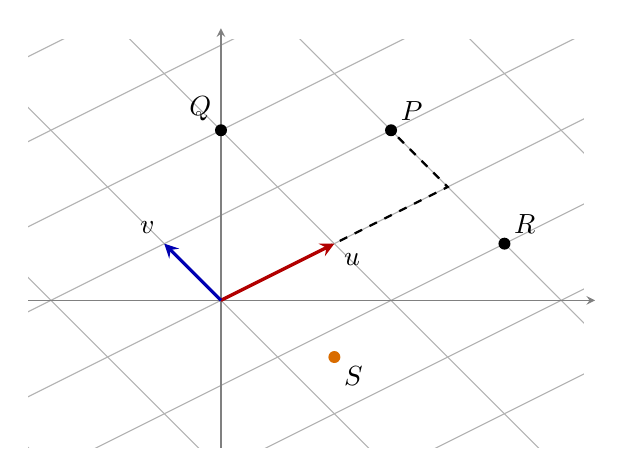
\begin{tikzpicture}[scale=0.72,>=stealth]
  \begin{scope}
    \clip (-3.4,-2.6) rectangle (6.4,4.6);
    \begin{scope}[cm={2,1,-1,1,(0,0)}]
      \foreach \k in {-6,...,6}{\draw[gray!60] (\k,-6)--(\k,6); \draw[gray!60] (-6,\k)--(6,\k);}
    \end{scope}
  \end{scope}
  \draw[->,gray] (-3.4,0)--(6.6,0); \draw[->,gray] (0,-2.6)--(0,4.8);
  \draw[dashed,thick] (0,0)--(4,2)--(3,3);
  \draw[->,very thick,red!70!black] (0,0)--(2,1);
  \draw[->,very thick,blue!70!black] (0,0)--(-1,1);
  \foreach \p in {(3,3),(0,3),(5,1)}{\fill \p circle (3pt);}
  \fill[orange!85!black] (2,-1) circle (3pt);
  \node[below right] at (2,1) {$u$};
  \node[above left] at (-1,1) {$v$};
  \node[above right] at (3,3) {$P$};
  \node[above left] at (0,3) {$Q$};
  \node[above right] at (5,1) {$R$};
  \node[below right] at (2,-1) {$S$};
\end{tikzpicture}
\end{center}

\textbf{Solution.} (a)~The grid lines are parallel to $\bv{u}$ and $\bv{v}$, so the weights of a corner are the numbers of steps along $\bv{u}$ and along $\bv{v}$ needed to reach it. For $P$, go two steps along $\bv{u}$ (to $(4,2)$, dashed) and one step along $\bv{v}$ (to $(3,3)$): the weights are $2$ and $1$. For $Q$, one step along $\bv{u}$ and two along $\bv{v}$ give $(2,1)+2(-1,1)=(0,3)$: the weights are $1$ and $2$. For $R$, two steps along $\bv{u}$ and one step \emph{backward} along $\bv{v}$ give $(4,2)-(-1,1)=(5,1)$: the weights are $2$ and $-1$. The point $S$ is not a corner of the grid. It sits inside a cell, so its weights are not whole numbers, and the picture alone cannot give them accurately.

(b)~By Theorem~\ref{thm:vecsys} each weight problem is a linear system with augmented matrix $[\bv{u}\ \bv{v}\ \bv{p}]$ for the point $\bv{p}$ in question. All four systems have the same coefficient matrix, so we row reduce once, with the four right-hand sides side by side:
\begin{align*}
&\begin{amat}{cc|cccc}2&-1&3&0&5&2\\1&1&3&3&1&-1\end{amat}
\rops{R_1\leftrightarrow R_2}
\begin{amat}{cc|cccc}1&1&3&3&1&-1\\2&-1&3&0&5&2\end{amat}\\[4pt]
&\rops{R_2-2R_1}
\begin{amat}{cc|cccc}1&1&3&3&1&-1\\0&-3&-3&-6&3&4\end{amat}
\rops{-\frac13R_2}
\begin{amat}{cc|cccc}1&1&3&3&1&-1\\0&1&1&2&-1&-\frac43\end{amat}\\[4pt]
&\rops{R_1-R_2}
\begin{amat}{cc|cccc}1&0&2&1&2&\frac13\\0&1&1&2&-1&-\frac43\end{amat}.
\end{align*}
Both columns on the left are pivot columns and no right-hand side column is a pivot column, so each of the four points is a linear combination of $\bv{u},\bv{v}$ with \emph{unique} weights. They are read from the columns on the right: $P$ has weights $(2,1)$, $Q$ has $(1,2)$, $R$ has $(2,-1)$, exactly as the picture suggested, and $S$ has $\bigl(\tfrac13,-\tfrac43\bigr)$. Check for $S$: $\tfrac13(2,1)-\tfrac43(-1,1)=\bigl(\tfrac23+\tfrac43,\ \tfrac13-\tfrac43\bigr)=(2,-1)$. \ $\checkmark$

\emph{Moral.} A picture is a fast way to find ``nice'' weights and to see why the answer is plausible. Row reduction finds the weights of \emph{every} point, including the ones the grid does not make visible, and it settles whether they are unique.
\end{exmp}

\begin{exmp}{Weights as formulas in the target}{bankFormula}
Let $\bv{a}_1=(2,3)$ and $\bv{a}_2=(1,2)$. (a)~Show that every vector $\bv{y}=(y_1,y_2)$ of $\R^2$ is a linear combination of $\bv{a}_1,\bv{a}_2$, and give the weights as formulas in $y_1$ and $y_2$. (b)~Use the formulas to write $(5,4)$ as a linear combination. (c)~What goes wrong if $\bv{a}_2$ is replaced by $(4,6)$?

\textbf{Solution.} (a)~Instead of one target, keep the target as unspecified numbers and row reduce once for all targets at the same time. The first two steps make the first pivot equal to $1$ without introducing fractions:
\begin{align*}
\begin{amat}{cc|c}2&1&y_1\\3&2&y_2\end{amat}
&\rops{R_2-R_1}
\begin{amat}{cc|c}2&1&y_1\\1&1&y_2-y_1\end{amat}
\rops{R_1\leftrightarrow R_2}
\begin{amat}{cc|c}1&1&y_2-y_1\\2&1&y_1\end{amat}\\[4pt]
&\rops{R_2-2R_1}
\begin{amat}{cc|c}1&1&y_2-y_1\\0&-1&3y_1-2y_2\end{amat}
\rops{-R_2}
\begin{amat}{cc|c}1&1&y_2-y_1\\0&1&-3y_1+2y_2\end{amat}\\[4pt]
&\rops{R_1-R_2}
\begin{amat}{cc|c}1&0&2y_1-y_2\\0&1&-3y_1+2y_2\end{amat}.
\end{align*}
Both columns are pivot columns and no row of zeros appeared, whatever $y_1,y_2$ are. So the system is consistent for every $\bv{y}$ and the weights are unique:
\[
x_1=2y_1-y_2,\qquad x_2=-3y_1+2y_2 .
\]
In particular $\Span\{\bv{a}_1,\bv{a}_2\}=\R^2$.

(b)~For $\bv{y}=(5,4)$ the formulas give $x_1=10-4=6$ and $x_2=-15+8=-7$. Check: $6(2,3)-7(1,2)=(12-7,\ 18-14)=(5,4)$. \ $\checkmark$

(c)~Now take $\bv{a}_2=(4,6)$. The same method, with a scaling step to avoid fractions, gives
\begin{align*}
\begin{amat}{cc|c}2&4&y_1\\3&6&y_2\end{amat}
&\rops{2R_2}
\begin{amat}{cc|c}2&4&y_1\\6&12&2y_2\end{amat}
\rops{R_2-3R_1}
\begin{amat}{cc|c}2&4&y_1\\0&0&2y_2-3y_1\end{amat}.
\end{align*}
The system is consistent if and only if $3y_1-2y_2=0$, so only the vectors on this line are combinations of $\bv{a}_1$ and $(4,6)$. This is no surprise: $(4,6)=2\bv{a}_1$, so the second vector repeats the first and the span is the single line through $\bv{0}$ and $(2,3)$ (compare Knowledge Check~\ref{kc:spans}(b)). And now the weights are not unique even when they exist, since the second column is not a pivot column.

\emph{Moral.} A row reduction with a symbolic target answers ``is \emph{every} target reachable?'' and ``what are the weights?'' in one pass. A zero row, with a condition on the $y_j$ attached to it, is what failure looks like.
\end{exmp}

\begin{exmp}{A blending problem with a free variable}{bankBlend}
Three dry foods are measured per serving by their protein, fat and fiber (in grams) and their energy (in units of $10$ kilocalories):
\[
\bv{f}_1=\begin{bmatrix}4\\1\\2\\3\end{bmatrix},\qquad
\bv{f}_2=\begin{bmatrix}1\\2\\3\\2\end{bmatrix},\qquad
\bv{f}_3=\begin{bmatrix}6\\5\\8\\7\end{bmatrix}.
\]
A daily ration must supply $16$\,g of protein, $11$\,g of fat, $18$\,g of fiber and $170$ kilocalories, that is $\bv{t}=(16,11,18,17)$. (a)~Find \emph{all} lists $(x_1,x_2,x_3)$ of numbers of servings with $x_1\bv{f}_1+x_2\bv{f}_2+x_3\bv{f}_3=\bv{t}$. (b)~Servings cannot be negative; which of the solutions are usable? (c)~What is the largest number of servings of Food~3 that a usable ration can contain?

\textbf{Solution.} (a)~By Theorem~\ref{thm:vecsys} we row reduce $[\bv{f}_1\ \bv{f}_2\ \bv{f}_3\ \bv{t}]$. There are four equations in three unknowns, but that does not decide anything by itself; the pivots do.
\begin{align*}
&\begin{amat}{ccc|c}4&1&6&16\\1&2&5&11\\2&3&8&18\\3&2&7&17\end{amat}
\rops{R_1\leftrightarrow R_2}
\begin{amat}{ccc|c}1&2&5&11\\4&1&6&16\\2&3&8&18\\3&2&7&17\end{amat}
\\[4pt]
&\rops{R_2-4R_1,\ R_3-2R_1,\ R_4-3R_1}
\begin{amat}{ccc|c}1&2&5&11\\0&-7&-14&-28\\0&-1&-2&-4\\0&-4&-8&-16\end{amat}
\rops{-\frac17R_2}
\begin{amat}{ccc|c}1&2&5&11\\0&1&2&4\\0&-1&-2&-4\\0&-4&-8&-16\end{amat}\\[4pt]
&\rops{R_3+R_2,\ R_4+4R_2}
\begin{amat}{ccc|c}1&2&5&11\\0&1&2&4\\0&0&0&0\\0&0&0&0\end{amat}
\rops{R_1-2R_2}
\begin{amat}{ccc|c}1&0&1&3\\0&1&2&4\\0&0&0&0\\0&0&0&0\end{amat}.
\end{align*}
The last column is not a pivot column, so the target can be met. Column $3$ is not a pivot column either, so $x_3$ is free (Definition~\ref{1.2-def:basicfree}) and the general solution is
\[
x_1=3-x_3,\qquad x_2=4-2x_3,\qquad x_3\ \text{free}.
\]
Check with $x_3=1$: $2\bv{f}_1+2\bv{f}_2+\bv{f}_3=(8+2+6,\ 2+4+5,\ 4+6+8,\ 6+4+7)=(16,11,18,17)$. \ $\checkmark$

(b)~The equations know nothing about the context, so we impose it: $x_1\ge0$ means $x_3\le3$, and $x_2\ge0$ means $x_3\le2$, and $x_3\ge0$ is required as well. All three hold exactly when $0\le x_3\le2$. So the usable rations are
\[
(x_1,x_2,x_3)=(3-t,\ 4-2t,\ t)\qquad\text{for }0\le t\le2 .
\]
For example $t=0$ gives $(3,4,0)$, $t=1$ gives $(2,2,1)$ and $t=2$ gives $(1,0,2)$. Values such as $t=2.5$ solve the \emph{equation} but give $x_2=-1$, which is not a ration.

(c)~The largest usable value is $t=2$: a ration of $1$ serving of Food~1, none of Food~2 and $2$ servings of Food~3. Check: $\bv{f}_1+2\bv{f}_3=(4+12,\ 1+10,\ 2+16,\ 3+14)=(16,11,18,17)$. \ $\checkmark$

\emph{Why there is a free variable.} Look at the foods themselves: $\bv{f}_1+2\bv{f}_2=(6,5,8,7)=\bv{f}_3$. Food~3 is a combination of the other two, so anything built with it can be built without it, at the price of changing the other weights. This is the situation of Pause and think~\ref{think:recipes}, now with four requirements instead of three. Four equations and three unknowns made it look overdetermined, yet the two zero rows in the reduction show that two of the equations were consequences of the others.
\end{exmp}

\subsection*{Bank: a parameter inside the vectors}

\begin{exmp}{A parameter that collapses the span}{bankCollapse}
Let $\bv{v}_1=(1,0,2)$ and $\bv{v}_2(h)=(1,h,2)$, which depends on a number $h$, and let $\bv{b}=(3,6,6)$, $\bv{c}=(3,0,6)$ and $\bv{d}=(3,6,7)$. For which values of $h$ is each of $\bv{b},\bv{c},\bv{d}$ in $\Span\{\bv{v}_1,\bv{v}_2(h)\}$? When are the weights unique?

\textbf{Solution.} In Example~\ref{ex:param} the parameter was in the target. Here it sits in a spanning vector, so $h$ changes the span itself, and we must be ready to look at special values of $h$ separately. Put the three targets side by side and reduce, treating $h$ as a number that has not been chosen:
\begin{align*}
\begin{amat}{cc|ccc}1&1&3&3&3\\0&h&6&0&6\\2&2&6&6&7\end{amat}
&\rops{R_3-2R_1}
\begin{amat}{cc|ccc}1&1&3&3&3\\0&h&6&0&6\\0&0&0&0&1\end{amat}.
\end{align*}
We read the three systems one at a time. A system is inconsistent exactly when its right-hand side column has a nonzero entry in a row whose left part is zero.

\emph{The vector $\bv{d}$.} Its column ends with the row $[\,0\ \ 0\mid1\,]$ whatever $h$ is, so $\bv{d}$ is in the span for \emph{no} value of $h$.

\emph{The case $h\neq0$.} The left part has two pivots. The third row is zero for $\bv{b}$ and $\bv{c}$, so both are in the span, with unique weights: for $\bv{b}$, $x_2=\tfrac6h$ and $x_1=3-\tfrac6h$; for $\bv{c}$, $x_2=0$ and $x_1=3$. For instance with $h=2$, $\bv{b}=0\cdot\bv{v}_1+3\bv{v}_2(2)$, and indeed $3(1,2,2)=(3,6,6)$. \ $\checkmark$

\emph{The case $h=0$.} Now $\bv{v}_2(0)=(1,0,2)=\bv{v}_1$ and the second row of the left part is zero. For $\bv{b}$ the second row reads $[\,0\ \ 0\mid6\,]$: inconsistent, so $\bv{b}$ is \emph{not} in the span. For $\bv{c}$ it reads $[\,0\ \ 0\mid0\,]$: consistent, with $x_2$ free ($x_1=3-x_2$), so $\bv{c}$ is in the span with infinitely many choices of weights, such as $(3,0)$ and $(2,1)$.

So $\bv{b}$ is in the span for every $h\neq0$ and for no other $h$; $\bv{c}$ is in the span for every $h$, with unique weights exactly when $h\neq0$; $\bv{d}$ is never in the span.

\emph{What is really going on.} Since $\bv{v}_2(h)-\bv{v}_1=(0,h,0)$, every combination $x_1\bv{v}_1+x_2\bv{v}_2(h)$ equals $(x_1+x_2)\bv{v}_1+x_2\,(0,h,0)$, and conversely. So for every $h\neq0$ the span is the \emph{same} plane, the one containing $(1,0,2)$ and $(0,1,0)$; its equation is $2y_1-y_3=0$. The vector $\bv{d}$ misses that plane ($2\cdot3-7=-1\neq0$) and the vectors $\bv{b},\bv{c}$ lie in it ($6-6=0$). At the single value $h=0$ the second vector stops pointing out of the line through $\bv{v}_1$ and the span collapses to that line. A parameter in a spanning vector usually matters only at the exceptional values where the span changes size.
\end{exmp}

\subsection*{Bank: the shape of a span}

\begin{exmp}{A line, a plane or all of $\R^3$?}{bankClassify}
Describe geometrically the span of each list of vectors in $\R^3$, and for the plane find its equation. (a)~$(1,2,-1),\ (2,4,-2),\ (-3,-6,3)$. \ (b)~$(1,0,2),\ (0,1,1),\ (2,3,7)$. \ (c)~$(1,1,0),\ (0,1,1),\ (1,0,1)$.

\textbf{Solution.} In every case put the vectors into the columns of a matrix and count pivots. A column without a pivot is a combination of the columns before it, as in Pause and think~\ref{think:recipes}, so it adds nothing new to the span; the number of pivots counts the vectors that do.

(a)~Each vector is a multiple of the first:
\begin{align*}
\begin{amat}{ccc}1&2&-3\\2&4&-6\\-1&-2&3\end{amat}
&\rops{R_2-2R_1,\ R_3+R_1}
\begin{amat}{ccc}1&2&-3\\0&0&0\\0&0&0\end{amat}.
\end{align*}
There is one pivot, in column $1$. The span is the line through the origin and $(1,2,-1)$.

(b)~Reducing the matrix of the three vectors:
\begin{align*}
\begin{amat}{ccc}1&0&2\\0&1&3\\2&1&7\end{amat}
&\rops{R_3-2R_1}
\begin{amat}{ccc}1&0&2\\0&1&3\\0&1&3\end{amat}
\rops{R_3-R_2}
\begin{amat}{ccc}1&0&2\\0&1&3\\0&0&0\end{amat}.
\end{align*}
There are two pivots, in columns $1$ and $2$, so the third vector is a combination of the first two: indeed $(2,3,7)=2(1,0,2)+3(0,1,1)$. The span is the plane through the origin, $(1,0,2)$ and $(0,1,1)$. To find its equation, ask which $\bv{y}=(y_1,y_2,y_3)$ are combinations of just those two vectors, keeping $\bv{y}$ symbolic as in Example~\ref{ex:cond}:
\begin{align*}
\begin{amat}{cc|c}1&0&y_1\\0&1&y_2\\2&1&y_3\end{amat}
&\rops{R_3-2R_1}
\begin{amat}{cc|c}1&0&y_1\\0&1&y_2\\0&1&y_3-2y_1\end{amat}
\rops{R_3-R_2}
\begin{amat}{cc|c}1&0&y_1\\0&1&y_2\\0&0&y_3-2y_1-y_2\end{amat}.
\end{align*}
The plane is $2y_1+y_2-y_3=0$. Check the third vector: $4+3-7=0$. \ $\checkmark$

(c)~Reducing the matrix of the three vectors:
\begin{align*}
\begin{amat}{ccc}1&0&1\\1&1&0\\0&1&1\end{amat}
&\rops{R_2-R_1}
\begin{amat}{ccc}1&0&1\\0&1&-1\\0&1&1\end{amat}
\rops{R_3-R_2}
\begin{amat}{ccc}1&0&1\\0&1&-1\\0&0&2\end{amat}.
\end{align*}
There is a pivot in every column \emph{and} in every row. A pivot in every row means that, whatever the right-hand side, the last column is never a pivot column (Theorem~\ref{1.2-thm:existuniq}), so every $\bv{y}$ in $\R^3$ is a combination of the three vectors. The span is all of $\R^3$.

\emph{Moral.} Three vectors in $\R^3$ can span a line, a plane or all of $\R^3$, and nothing in the list of numbers shows which. The pivots do: one, two or three.
\end{exmp}

\begin{exmp}{Two conditions on a vector in $\R^4$}{bankTwoCond}
Let $\bv{w}_1=(1,2,0,1)$ and $\bv{w}_2=(0,1,1,-1)$ in $\R^4$. (a)~For which $\bv{y}=(y_1,y_2,y_3,y_4)$ is $\bv{y}$ in $\Span\{\bv{w}_1,\bv{w}_2\}$? (b)~Decide whether $\bv{p}=(2,7,3,-1)$, $\bv{q}=(1,2,0,0)$ and $\bv{r}=(1,2,5,1)$ are in the span, and give weights where they are. (c)~Why are there two conditions?

\textbf{Solution.} (a)~Row reduce $[\bv{w}_1\ \bv{w}_2\ \bv{y}]$ with $\bv{y}$ left symbolic:
\begin{align*}
\begin{amat}{cc|c}1&0&y_1\\2&1&y_2\\0&1&y_3\\1&-1&y_4\end{amat}
&\rops{R_2-2R_1,\ R_4-R_1}
\begin{amat}{cc|c}1&0&y_1\\0&1&y_2-2y_1\\0&1&y_3\\0&-1&y_4-y_1\end{amat}\\[4pt]
&\rops{R_3-R_2,\ R_4+R_2}
\begin{amat}{cc|c}1&0&y_1\\0&1&y_2-2y_1\\0&0&y_3-y_2+2y_1\\0&0&y_4+y_2-3y_1\end{amat}.
\end{align*}
Both columns on the left are pivot columns, and the two rows below them are zero rows on the left. The system is consistent if and only if \emph{both} of the entries on the right vanish:
\[
2y_1-y_2+y_3=0\qquad\text{and}\qquad -3y_1+y_2+y_4=0 .
\]
When they hold, the first two rows give the weights: $x_1=y_1$ and $x_2=y_2-2y_1$.

(b)~Test each vector against both equations.
\begin{itemize}
  \item $\bv{p}=(2,7,3,-1)$: $\ 4-7+3=0$ and $-6+7-1=0$. Both hold, so $\bv{p}$ is in the span, with weights $x_1=2$ and $x_2=7-4=3$. Check: $2(1,2,0,1)+3(0,1,1,-1)=(2,\ 7,\ 3,\ -1)$. \ $\checkmark$
  \item $\bv{q}=(1,2,0,0)$: $\ 2-2+0=0$ holds, but $-3+2+0=-1\neq0$. Only the first condition holds, so $\bv{q}$ is \emph{not} in the span.
  \item $\bv{r}=(1,2,5,1)$: $\ 2-2+5=5\neq0$, although $-3+2+1=0$. Only the second condition holds, so $\bv{r}$ is \emph{not} in the span.
\end{itemize}
So passing one test is not enough: each condition removes some vectors, and it takes both to describe the span.

(c)~A vector in the span is $x_1\bv{w}_1+x_2\bv{w}_2=(x_1,\ 2x_1+x_2,\ x_2,\ x_1-x_2)$: two free numbers fill four coordinates, so two coordinates are determined by the others, and that is what two equations say. In terms of pivots: the matrix $[\bv{w}_1\ \bv{w}_2]$ has $4$ rows but only $2$ pivots, so $4-2=2$ rows end up as zero rows, and each gives one condition. In $\R^3$ the span of two vectors needed one condition (Example~\ref{ex:cond}); in $\R^4$ it needs two. (This is the idea behind Pause and think~\ref{think:howmany}: two vectors are far too few to fill $\R^4$.)
\end{exmp}

\subsection*{Answers and discussion}
\begin{description}[leftmargin=0pt,itemsep=5pt]
  \item[Knowledge Check \ref{kc:compute}.] $3\bv{u}+2\bv{v}=(6,-3)+(-2,6)=(4,3)$ and $\bv{u}-\bv{v}=(2-(-1),\,-1-3)=(3,-4)$.
  \item[Knowledge Check \ref{kc:vecequal}.] The left side is $(x+y,\ x-y)$. Two vectors are equal exactly when their entries are equal, so
        $x+y=5$ and $x-y=1$. Adding gives $2x=6$, so $x=3$ and $y=2$. Check: $3(1,1)+2(1,-1)=(5,1)$. \ $\checkmark$ (A vector equation is
        a system in disguise, which is the idea of this whole section.)
  \item[Knowledge Check \ref{kc:augmatrix}.] The vectors become the columns, in order, followed by the right-hand side:
        $\begin{amat}{cc|c}1&3&-1\\0&2&5\\-4&0&7\end{amat}$. The equivalent system is $x_1+3x_2=-1$, \ $2x_2=5$, \ $-4x_1=7$.
  \item[Knowledge Check \ref{kc:spans}.] (a)~The line through the origin and $(2,-4)$, i.e.\ the line $y=-2x$.
        (b)~Since $(-3,-6)=-3(1,2)$, the second vector adds nothing: the span is the line through the origin and $(1,2)$.
        (c)~All of $\R^2$: any $(a,b)$ equals $a(1,0)+b(0,1)$. (d)~Only the single point $\bv{0}$.
  \item[Knowledge Check \ref{kc:member}.] $(6,-3,9)=3\cdot(2,-1,3)$, so yes. $(1,0,0)$ is not in $\Span\{(0,1,0),(0,0,1)\}$: every vector in that
        span has first entry $0\cdot$(anything)$+\,0\cdot$(anything)$\,=0$.
  \item[Pause and think \ref{think:axioms}.] A new collection of objects needs a sum and a scalar multiple that obey \emph{all eight} rules (and be closed under
        the two operations, meaning the results stay inside the collection). Nothing special about columns of numbers is used elsewhere.
        For polynomials of degree at most $2$, add coefficient by coefficient; all eight rules hold, so these
        polynomials ``behave like'' $\R^3$ in every respect we use, even though they are not columns. Section~4.1 will define a
        \emph{vector space} as any collection with operations satisfying these rules. For the positive vectors in $\R^2$: sums of
        positive vectors are positive, but there is no zero vector in the collection (rule (iii) has nothing to point to), no negatives
        (rule (iv) fails), and $(-1)(1,1)$ leaves the collection. So the collection is not closed under scalar multiplication.
  \item[Pause and think \ref{think:arrow}.] The picture is a faithful model for $\R^2$ and $\R^3$, where the arrow for the sum, difference or
        multiple is exactly what the entrywise formula says. In $\R^5$ the algebra is the same entry-by-entry computation,
        so we use the pictures in $\R^2$ and $\R^3$ as guides for \emph{what to expect} and the algebra as the \emph{proof}. A vector is
        determined by its entries, not by where an arrow starts: the arrows from $\bv{0}$ to $\bv{u}$ and from $\bv{v}$ to $\bv{u}+\bv{v}$ are
        parallel copies of one vector. For $\bv{u}=(2,1)$ and $\bv{v}=(1,3)$ we get $\bv{u}-\bv{v}=(1,-2)$, which is the vector that points \emph{from the
        tip of $\bv{v}$ to the tip of $\bv{u}$} (check: $\bv{v}+(\bv{u}-\bv{v})=\bv{u}$). It is also the fourth vertex of the parallelogram with vertices
        $\bv{0},\bv{u},-\bv{v}$.
  \item[Pause and think \ref{think:recipes}.] Since $\bv{v}_3=(1,1,2)=\bv{v}_1+\bv{v}_2$, the equation
        $1\bv{v}_1+1\bv{v}_2-1\bv{v}_3=\bv{0}$ holds. Adding any multiple $t$ of this relation to one list of weights gives another list that produces the same vector:
        $(x_1,x_2,x_3)\mapsto(x_1+t,\,x_2+t,\,x_3-t)$. That is exactly the freedom $x_1=2-x_3$, $x_2=3-x_3$ in the
        free variable. The vector $\bv{v}_3$ is redundant: anything made with $\bv{v}_3$ can be made without it. If $\bv{v}_3$ were not a combination of
        $\bv{v}_1,\bv{v}_2$, the third column would be a pivot column, there would be no free variable, and the weights would be forced, as in
        Example~\ref{ex:inspan}. Redundancy of vectors within a list is the idea of \emph{linear dependence}, taken up in Section~1.7.
  \item[Pause and think \ref{think:closure}.] Write $\bv{u}=c_1\bv{w}_1+c_2\bv{w}_2+c_3\bv{w}_3$ and $\bv{v}=d_1\bv{w}_1+d_2\bv{w}_2+d_3\bv{w}_3$. Then
        $\bv{u}+\bv{v}=(c_1+d_1)\bv{w}_1+(c_2+d_2)\bv{w}_2+(c_3+d_3)\bv{w}_3$ and
        $5\bv{u}=(5c_1)\bv{w}_1+(5c_2)\bv{w}_2+(5c_3)\bv{w}_3$, using Theorem~\ref{thm:props}(vi), (vii) and (ii). Both are again of the form
        $(\text{scalar})\bv{w}_1+(\text{scalar})\bv{w}_2+(\text{scalar})\bv{w}_3$. So adding vectors of a span, or scaling them, never takes you out of the span.
        A circle $x_1^2+x_2^2=1$ fails: $(1,0)$ and $(0,1)$ are on it but $(1,0)+(0,1)=(1,1)$ is not, and $2(1,0)=(2,0)$ is not.
        Sets with this ``closed'' property will be called \emph{subspaces} in Section~4.1; every span is one.
  \item[Pause and think \ref{think:howmany}.] Two vectors in $\R^3$ cannot span $\R^3$. The matrix $[\,\bv{v}_1\ \bv{v}_2\,]$ is $3\times2$, so it has at most $2$
        pivot positions but $3$ rows, so some row has no pivot; by Theorem~\ref{1.2-thm:counting}(d) there is a vector $\bv{b}$ for which the system is
        inconsistent. (In Example~\ref{ex:cond} that vector was $\bv{c}=(5,0,-6)$.) The same argument works for $p$ vectors in $\R^m$ whenever $p<m$:
        a matrix with $m$ rows and $p<m$ columns cannot have a pivot in every row. So \emph{at least $m$ vectors are needed to span $\R^m$.}
        The number alone is not enough: $(1,2)$ and $(2,4)$ are two vectors in $\R^2$ but span only a line, since the second is a multiple of the first.
        Whether enough vectors \emph{do} span is a question about pivots; Section~1.4 makes the connection exact.
  \item[Pause and think \ref{think:feasible}.] The three requirements were not independent: the target is a combination of the two food vectors, equivalently it lies in the
        plane spanned by them. Changing the fiber target to $8$ g gives the augmented matrix
        $\begin{amat}{cc|c}100&50&250\\4&1&9\\2&3&8\end{amat}$, which row reduces (with the same steps as before, ending with $R_3-R_1$ and $R_3+2R_2$) to a row $[\,0\ \ 0\mid1\,]$ with a nonzero
        entry in the last column. So the target $(250,9,8)$ is \emph{not} in the span, and no combination of the two foods produces it: a third food or a different target is needed.
        The equation itself does not know that servings cannot be negative; it is pure algebra. A solution with $x_1<0$ would be a consistent answer to the \emph{equation} but a
        useless answer to the \emph{problem}. Modeling always requires checking the answer against the context.
  \item[Before the next section.] (1)~A single nonzero vector spans a line. Two vectors in $\R^3$ span a plane through the origin (example: $(1,0,0),(0,1,0)$), a line
        (example: $(1,2,3),(2,4,6)$), or just $\{\bv{0}\}$ (example: $\bv{0},\bv{0}$). They cannot span $\R^3$. (2)~Because it packages a whole
        vector equation into a single expression that depends only on the matrix and the list of weights, so the equation becomes
        ``$(\text{matrix})\cdot(\text{unknown list})=\bv{b}$'', which looks like $ax=b$ for numbers. (3)~False.
        With $\bv{a}_1=(1,2)$, $\bv{a}_2=(2,4)$ and $\bv{b}=(3,6)$ we have $\bv{b}=3\bv{a}_1+0\bv{a}_2=1\bv{a}_1+1\bv{a}_2$.
\end{description}

\end{document}
